\graphicspath{ {./content/simu/figure/} }

\section{Random walk and PSO}\label{sec:3}

Random walk is compared to PSO with two degrees of freedom. Tow point was compared, one is the time commutation and the second is the coverage rate.
The experimentation is implemented by using Matlab to compute the position of cameras and optimize it with the PSO algorithm (toolbox PSO \cite{matlab,vrep}) and random walk.
The first experiment shows the efficiency of PSO compared to random walk for cover an area ( see figure 3 and figure 5) but the speed (number of iterations ) is much longer with PSO to Random walk (see figure 4  and figure6)   

\subsection{Random walk }\label{subsec:31}

The first experiment use a basic algorithm. The random walk work with successive selection of random solution, try it and if the solution is better to the precedent solution this is the new reference. If after 100 test (figure 4) the solution was not better, the algorithm stop and give the final solution. 
	This basic algorithm give some result, and this result is the point of reference for the other algorithm 
 %% figure3 fig3.png
 %%Figure 3: Percentage of coverage with n number of camera (1 to 20). The camera was positioning with basic Random Walk algorithm for optimize the position on X and Y pose
\begin{figure}
  \centering
  \hspace*{\fill}
  %\subfigure[]{\label{subfig:4a}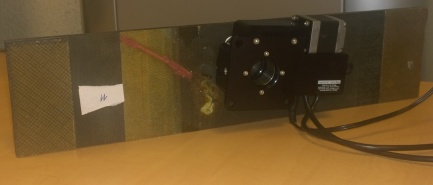
\includegraphics[width=0.3\linewidth]{fig4a.png}} \hfill
  %\subfigure[]{\label{subfig:4b}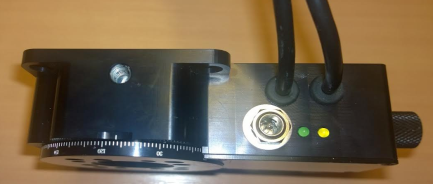
\includegraphics[width=0.3\linewidth]{fig4b.png}} 
  %\hspace*{\fill} \\ \hspace*{\fill}
  %\subfigure[]{\label{subfig:4c}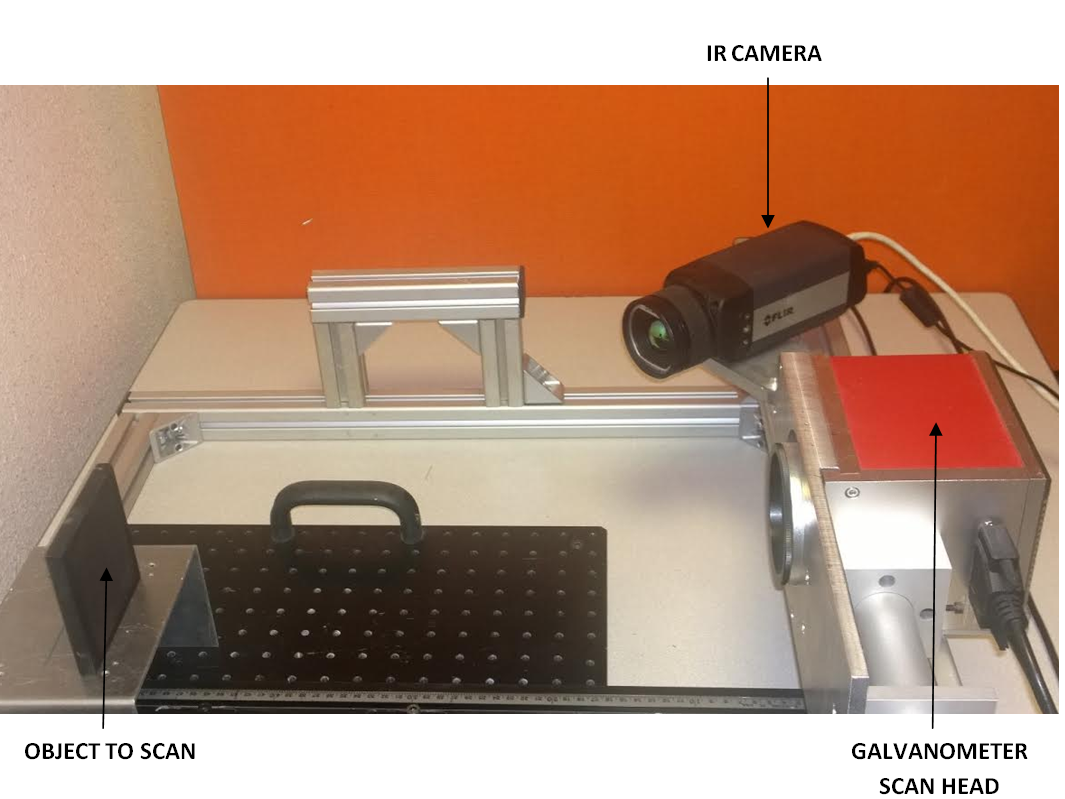
\includegraphics[width=0.3\linewidth]{fig4c.png}}
	.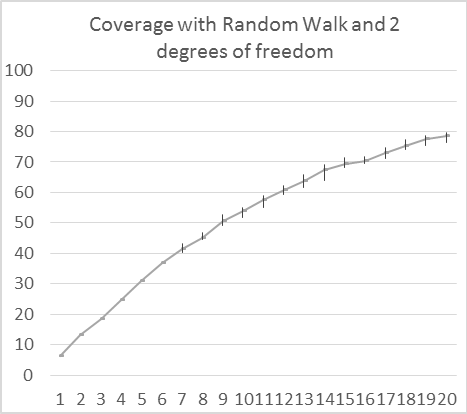
\includegraphics[width=0.7\linewidth]{fig3.png}
  \hspace*{\fill}
  \caption{%(a)-(b) Device for positioning the composite material - 
	Percentage of coverage with n number of camera (1 to 20). The camera was positioning with basic Random Walk algorithm for optimize the position on X and Y pose  }
  \label{fig:422}
\end{figure}
 %% figure4 fig4.png
 %%Figure 4: Number of iterations before converged solution.  The algorithm implement for the random walk stop when it’s impossible to find best solution after 100 random set of camera pose.  
 \begin{figure}
  \centering
  \hspace*{\fill}
  %\subfigure[]{\label{subfig:4a}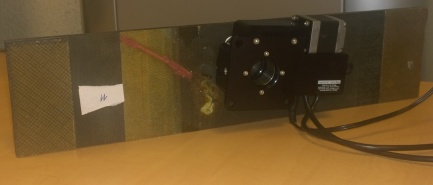
\includegraphics[width=0.3\linewidth]{fig4a.png}} \hfill
  %\subfigure[]{\label{subfig:4b}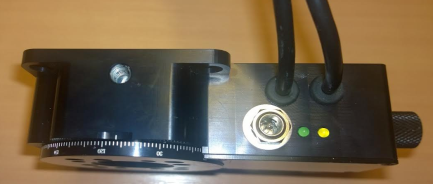
\includegraphics[width=0.3\linewidth]{fig4b.png}} 
  %\hspace*{\fill} \\ \hspace*{\fill}
  %\subfigure[]{\label{subfig:4c}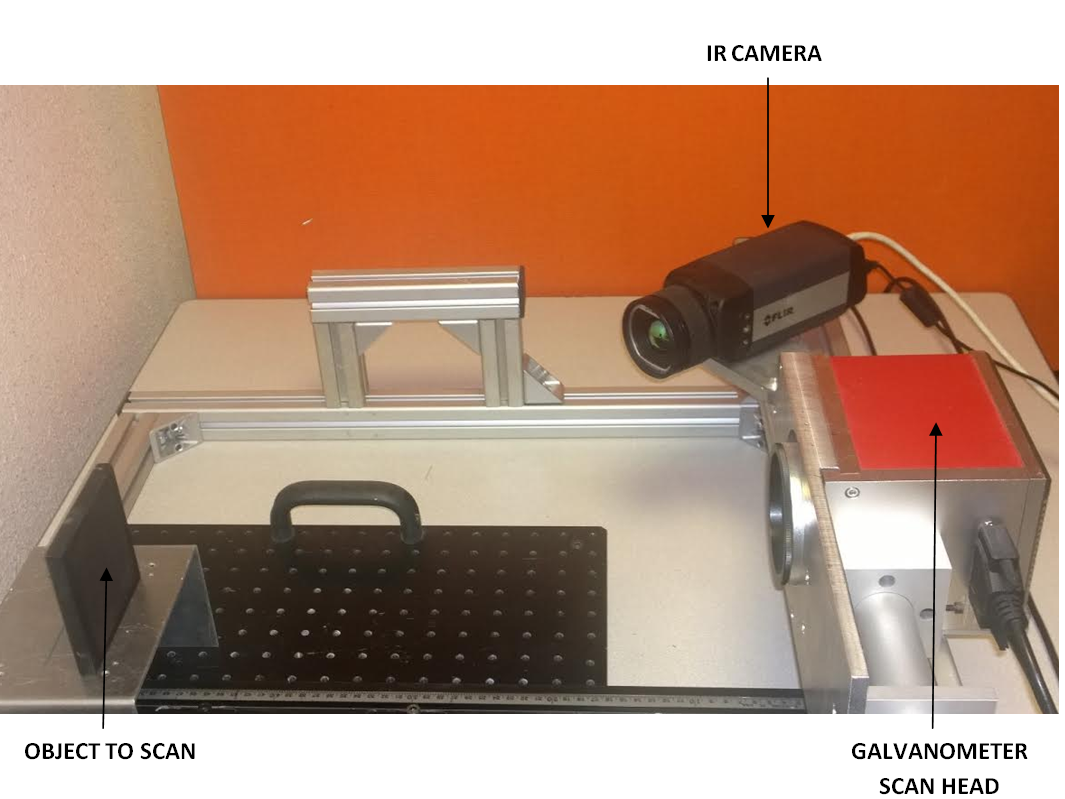
\includegraphics[width=0.3\linewidth]{fig4c.png}}
	.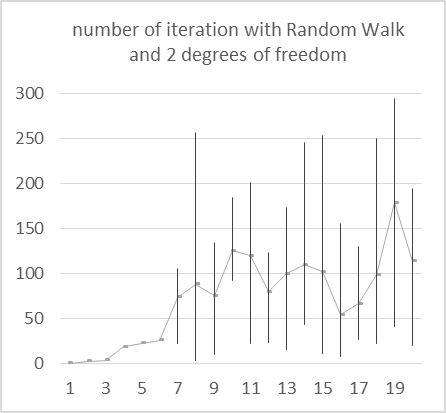
\includegraphics[width=0.7\linewidth]{fig4.png}
  \hspace*{\fill}
  \caption{%(a)-(b) Device for positioning the composite material - 
	Number of iterations before converged solution.  The algorithm implement for the random walk stop when it’s impossible to find best solution after 100 random set of camera pose. }
  \label{fig:422}
\end{figure}
 The limit of the random walk is at the first the result proposed was not enough efficient (figure 3) and at same time, many gap appear between the results with the same input parameter (the gap vary between 2 percentages point to 5 percentages point). The other limit of the random walk is time computation (figure 4) with big gap between the min number of iteration and the max and the time computation increase really fast despite the little number of camera. The problem caused by the time computation can be a curb for the future deployment for an adaptive camera network. Now the limit of random walk was clearly identify it’s important to find a better algorithm.  
 
\subsubsection{PSO with 2 degrees of freedom}\label{subsec:311}

%% fig 5  fig5.png
%%Figure 5: Percentage of coverage with n number of camera (1 to 20). The camera was positioning with PSO algorithm for optimize the position on X and Y pose.  
\begin{figure}
  \centering
  \hspace*{\fill}
  %\subfigure[]{\label{subfig:4a}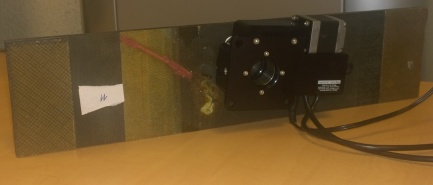
\includegraphics[width=0.3\linewidth]{fig4a.png}} \hfill
  %\subfigure[]{\label{subfig:4b}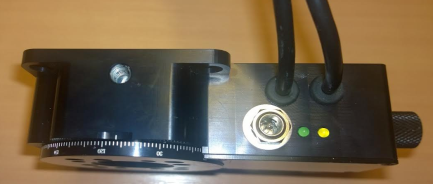
\includegraphics[width=0.3\linewidth]{fig4b.png}} 
  %\hspace*{\fill} \\ \hspace*{\fill}
  %\subfigure[]{\label{subfig:4c}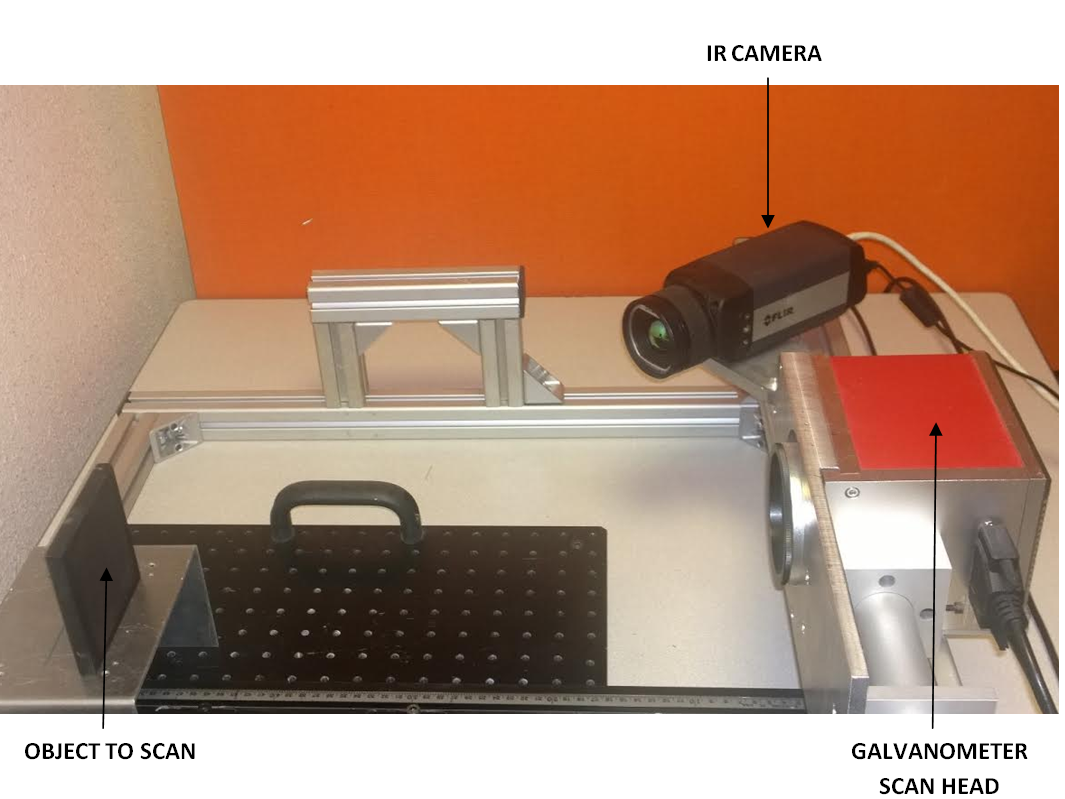
\includegraphics[width=0.3\linewidth]{fig4c.png}}
	.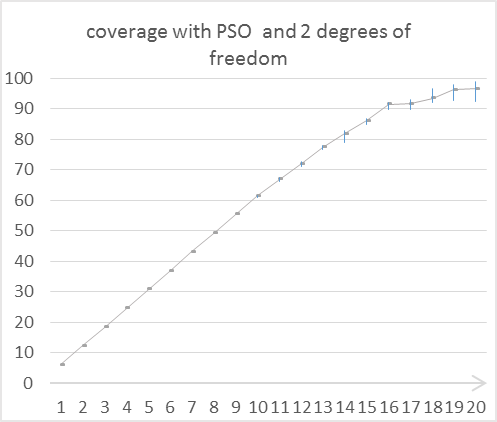
\includegraphics[width=0.7\linewidth]{fig5.png}
  \hspace*{\fill}
  \caption{%(a)-(b) Device for positioning the composite material - 
	Percentage of coverage with n number of camera (1 to 20). The camera was positioning with PSO algorithm for optimize the position on X and Y pose.  }
  \label{fig:422}
\end{figure}
%% fig 6  fig65.png
%%Figure 6: Number of iterations before converged solution.  The algorithm implement for the PSO stop when it’s impossible to find best solution after 100 random set of camera pose.  .

\begin{figure}
  \centering
  \hspace*{\fill}
  %\subfigure[]{\label{subfig:4a}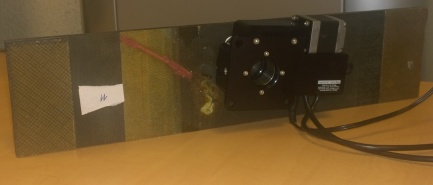
\includegraphics[width=0.3\linewidth]{fig4a.png}} \hfill
  %\subfigure[]{\label{subfig:4b}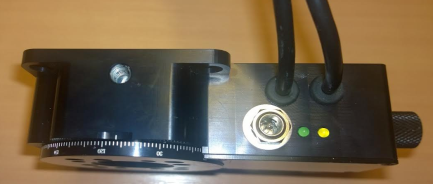
\includegraphics[width=0.3\linewidth]{fig4b.png}} 
  %\hspace*{\fill} \\ \hspace*{\fill}
  %\subfigure[]{\label{subfig:4c}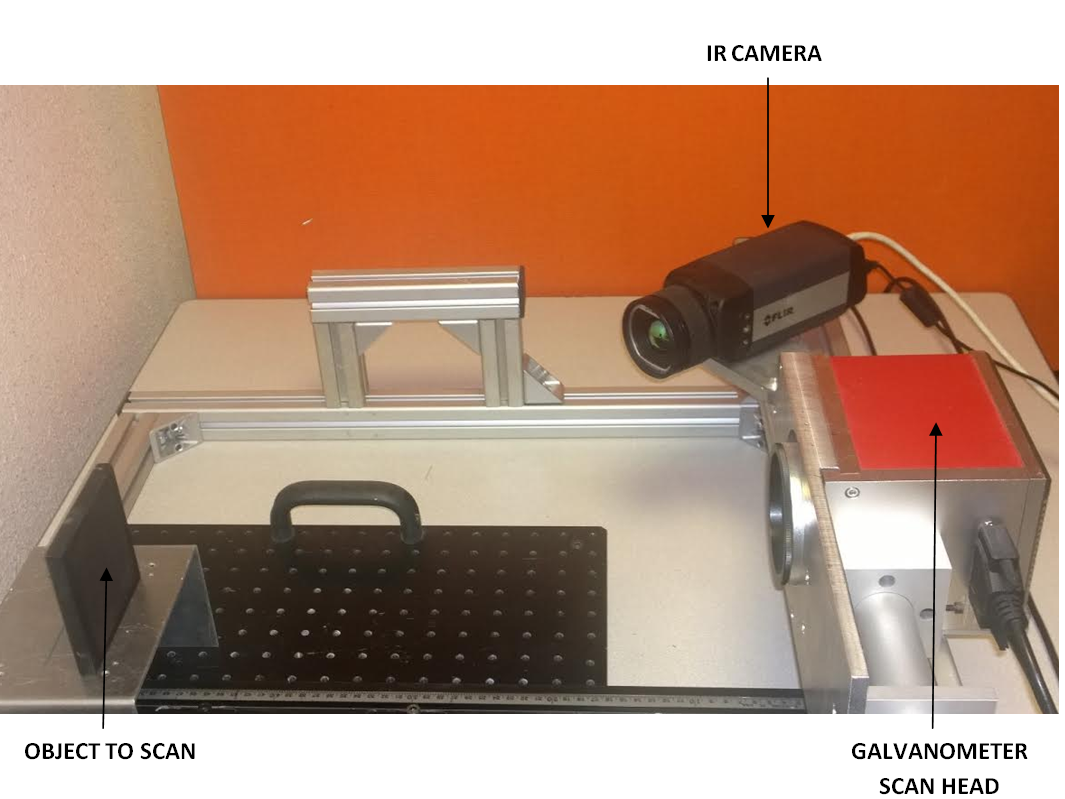
\includegraphics[width=0.3\linewidth]{fig4c.png}}
	.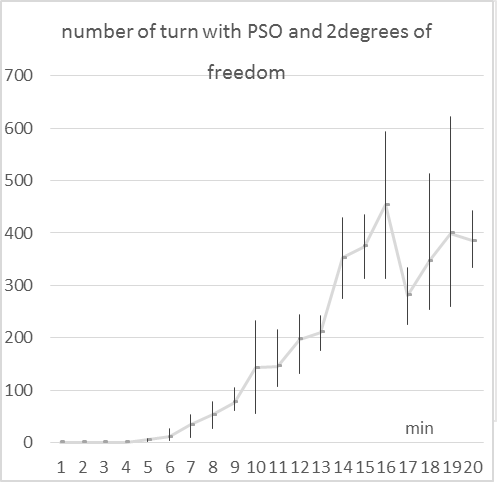
\includegraphics[width=0.7\linewidth]{fig6.png}
  \hspace*{\fill}
  \caption{%(a)-(b) Device for positioning the composite material - 
	 Number of iterations before converged solution.  The algorithm implement for the PSO stop when it’s impossible to find best solution after 100 random set of camera pose.}
  \label{fig:422}
\end{figure}
Comparing the results obtained with the two algorithms (random walk and PSO) allows to evidence that Although the random walk is 2 time faster (see figure 4 and figure 6)for all size of the network camera, but the coverage proposed by the random walk is not acceptable and use too many camera for a complete coverage of the room, (see fig 5 and figure 6) more even if the PSO make more time the result is much better and can have the complete coverage with one smaller camera network and for any number of camera you have best result with PSO.
But the number of cameras is too much important and to try to down the number of sensors used on the network, is possible to add one more degrees of freedom. 




%%% Local Variables: 
%%% mode: latex
%%% TeX-master: "../../master"
%%% End: 
